% !Mode:: "TeX:UTF-8"
% !TEX program  = xelatex

% 模板名称:YangThesis
% 模板版本:V1.0
% 模板作者:JingXuan Yang
% 联系作者:yangjingxuan@stu.hit.edu.cn
% 模板来源:数模竞赛模板的二次开发
% 模板适用:普通课程论文,略作修改可用作毕业设计(论文)
% 模板编译:XeLaTeX,编译两次,两次,两次!!!
% 更新时间:4/14/2019
% 模板说明:本模板尽量把接口留在了类文件外面,但是顾名思义,模板即为
%                 部分样式的集合,有些样式是定义在类文件里面的,在外面无法
%                 修改。类文件中注释齐全,很多样式可以个性化定义,建议拥有
%                 一定LaTeX基础以后再尝试修改类文件(YangThesis.cls)。

% 本模板提供有、无封面两种选择
% 1、采用封面
% 模板默认采用封面
% no-math选项指不采用模板文件对数学符号字体的定义
% 可在settings.tex里设置数学符号字体
 \documentclass[no-math]{YangThesis} 

% 2、去掉封面,添加<withoutpreface>选项
%\documentclass[no-math, withoutpreface]{YangThesis} 

% 导入配置文件settings.tex,
% 配置参数均存储在settings.tex文件中,
% 添加或修改均需在该文件中进行
% 注意:页眉页脚的设计也在此文件中
% settings.tex
% YangTemplate.cls 的配置文件
% 采用<\input>放入主文档中,不可单独编译

\usepackage[T1]{fontenc}

% 正文和数学字体均采用Times New Roman字体
% \usepackage{newtxtext, newtxmath}

% 只正文采用Times字体,数学公式保持默认字体
\usepackage{newtxtext}

\usepackage{float}

% 定制tikz流程图形状
\usepackage{tikz}
\usetikzlibrary{shapes.geometric, arrows}
% 开始
\tikzstyle{startstop} = [rectangle, rounded corners, minimum width = 2cm, minimum height=1cm,text centered, draw = black]
% 输入输出
\tikzstyle{io} = [trapezium, trapezium left angle=70, trapezium right angle=110, minimum width=2cm, minimum height=1cm, text centered, draw=black]
% 过程
\tikzstyle{process} = [rectangle, minimum width=3cm, minimum height=1cm, text centered, draw=black]
% 判断
\tikzstyle{decision} = [diamond, aspect = 3, text centered, draw=black]
% 箭头形式
\tikzstyle{arrow} = [->,>=stealth]

% 设置编号格式
\newcounter{rowno}
\numberwithin{equation}{section}
\numberwithin{figure}{section}
\numberwithin{table}{section}
\renewcommand{\thefigure}{\arabic{section}-\arabic{figure}}
\renewcommand{\thetable}{\arabic{section}-\arabic{table}}
\renewcommand{\theequation}{\arabic{section}-\arabic{equation}}

% 新数学命令
\newcommand\dif{\mathrm{d}}
\newcommand\no{\noindent}
\newcommand\dis{\displaystyle}
\newcommand\ls{\leqslant}
\newcommand\gs{\geqslant}

\newcommand\limit{\dis\lim\limits}
\newcommand\limn{\dis\lim\limits_{n\to\infty}}
\newcommand\limxz{\dis\lim\limits_{x\to0}}
\newcommand\limxi{\dis\lim\limits_{x\to\infty}}
\newcommand\limxpi{\dis\lim\limits_{x\to+\infty}}
\newcommand\limxni{\dis\lim\limits_{x\to-\infty}}

% 默认上限为无穷
\newcommand\sumnf{\dis\sum\limits_{n=1}^{\infty}}
\newcommand\sumnz{\dis\sum\limits_{n=0}^{\infty}}
\newcommand\sumkf{\dis\sum\limits_{k=1}^{\infty}}
\newcommand\sumkz{\dis\sum\limits_{k=0}^{\infty}}
\newcommand\sumifn{\dis\sum\limits_{i=1}^{n}}
\newcommand\sumizn{\dis\sum\limits_{i=0}^{n}}
\newcommand\sumkzn{\dis\sum\limits_{k=0}^n}
\newcommand\sumkfn{\dis\sum\limits_{k=1}^n}

\newcommand\pzx{\dis\frac{\partial z}{\partial x}}
\newcommand\pzy{\dis\frac{\partial z}{\partial y}}

\newcommand\pfx{\dis\frac{\partial f}{\partial x}}
\newcommand\pfy{\dis\frac{\partial f}{\partial x}}

\newcommand\pzxx{\dis\frac{\partial^2 z}{\partial x^2}}
\newcommand\pzxy{\dis\frac{\partial^2 z}{\partial x\partial y}}
\newcommand\pzyx{\dis\frac{\partial^2 z}{\partial y\partial x}}
\newcommand\pzyy{\dis\frac{\partial^2 z}{\partial y^2}}

\newcommand\pfxx{\dis\frac{\partial^2 f}{\partial x^2}}
\newcommand\pfxy{\dis\frac{\partial^2 f}{\partial x\partial y}}
\newcommand\pfyx{\dis\frac{\partial^2 f}{\partial y\partial x}}
\newcommand\pfyy{\dis\frac{\partial^2 f}{\partial y^2}}

\newcommand\intzi{\dis\int_{0}^{+\infty}}
\newcommand\intd{\dis\int}
\newcommand\intab{\dis\int_a^b}

\newcommand\mc{\mathbb{C}}
\newcommand\mr{\mathbb{R}}
\newcommand{\degree}{^\circ}

\newenvironment{mfrac}[2]%
{\raise0.5ex\hbox{$#1$}\! \left/ \! \lower0.5ex\hbox{$#2$}\right.}

% 定义新数学符号
\DeclareMathOperator{\sgn}{sgn}
\DeclareMathOperator{\arccot}{arccot}
\DeclareMathOperator{\arccosh}{arccosh}
\DeclareMathOperator{\arcsinh}{arcsinh}
\DeclareMathOperator{\arctanh}{arctanh}
\DeclareMathOperator{\arccoth}{arccoth}
\DeclareMathOperator{\grad}{\bf{grad}}
\DeclareMathOperator{\diag}{diag}
\DeclareMathOperator{\csign}{csign}

\usepackage{url}

% 自定义字号大小命令
% 修改18pt为想要的字号即可
\newcommand{\myfont}{\fontsize{18pt}{\baselineskip}\selectfont}

% 参考文献标号为上标
\newcommand{\upcite}[1]{\textsuperscript{\textsuperscript{\cite{#1}}}}

% 定制页眉页脚
\usepackage{fancyhdr}
\pagestyle{fancy}
% 页眉
\lhead{}
\chead{MEMS计算机辅助设计研究现状综述}
\rhead{}
% 页脚
\lfoot{}
\cfoot{-\thepage-}
\rfoot{}

% 页眉页脚单横线
%\renewcommand{\headrulewidth}{0.4pt}
%\renewcommand{\footrulewidth}{0pt}

% 页眉双横线
\newcommand{\makeheadrule}{%
\makebox[0pt][l]{\rule[0.2\baselineskip]{\headwidth}{1.3pt}}%
\rule[0.35\baselineskip]{\headwidth}{2.5pt}}
\renewcommand{\headrule}{%
{\if@fancyplain\let\headrulewidth\plainheadrulewidth\fi
\makeheadrule}}
\makeatother

% 设置脚注编号格式
\renewcommand{\thefootnote}{\fnsymbol{footnote}}



% 封面信息
% 论文类别
\papercategory{CAD/CAM技术基础课程论文}
% 论文标题
\title{MEMS计算机辅助设计研究现状综述}
% 学校名称
\schoolname{哈尔滨工业大学(深圳)}
% 学院名称
\departname{机电工程与自动化学院}
% 专业
\majorin{机械类}
% 班级
\classnumber{机械二班}
% 姓名
\authorname{杨敬轩}
% 学号
\studentID{SZ160310217}
% 日期
\dateinput{2019年04月17日}

%%%=====================%%%
% 开始写文章
\begin{document}

% 生成标题
\maketitle

% 页码从1开始计数
\setcounter{page}{1}
% 页码采用罗马数字格式
\pagenumbering{Roman}
 
% 开始写摘要
\begin{abstract}
% 将摘要添加到目录中,<\,>为添加水平间距的命令
\addcontentsline{toc}{section}{摘\,\,要}
 
MEMS 是一个多能量域耦合、多学科交叉的复杂系统,一个成功的 MEMS 设计必须借助于计算机辅助设计。本文结合国内、国际 MEMS 计算机辅助设计的最新成果,对 MEMS 的概念、MEMS CAD的概念、研究MEMS CAD的意义、MEMS计算机建模与仿真四个级别的方法及其技术进行了详细的论述。在前述分析的基础上,本文总结了MEMS CAD研究的关键性科学技术问题,对当前MEMS CAD的研究中存在的问题和MEMS CAD未来的发展趋势进行了深入地思考和讨论。本文对 MEMS 器件或系统设计以及 MEMS CAD 的研究具有参考价值。

% 中文关键词
\keywords{MEMS CAD;MEMS;计算机辅助设计;研究现状综述}
\end{abstract}

% 英文摘要
\begin{abstracten}
\addcontentsline{toc}{section}{Abstract}

MEMS is a multi-energy-domain coupled and multidisciplinary complex system. A successful MEMS design must rely on computer-aided design. This paper combines the latest achievements of domestic and international MEMS computer-aided design, and discusses the concept of MEMS and MEMS CAD, the research value  of MEMS CAD, and the four concepts and techniques of MEMS computer modeling and simulation. Based on the above analysis, this paper summarizes the key scientific and technical issues of MEMS CAD research, and deeply considers and discusses the problems existing in the current research of MEMS CAD and the future development trend of MEMS CAD. This paper has reference value for MEMS device or system design and MEMS CAD research.

% 英文关键词
\keywordsen{MEMS CAD; MEMS; CAD; Summary of research status}
\end{abstracten}

% 强制目录二字位于最上方,距离可调
% 模板不完善,暂采取此方法
\vspace{-1.3cm}

% 生成目录
\tableofcontents
% 将目录项添加到目录中
\addcontentsline{toc}{section}{目\,\,录}

% 分页,撰写正文
\clearpage
% 调整标题与上边的距离
\vspace{-1cm}
% 第1章的标题
\section{MEMS CAD的技术背景}

% 页码从1开始计数
\setcounter{page}{1}
% 页码格式采用阿拉伯数字
\pagenumbering{arabic}

% 正文内容,注意LaTeX分段有两种方法,直接空一行或者使用<\par>
% 默认首行缩进,不需要在代码编辑区手动敲空格
\subsection{MEMS概述}
微机电系统 (MEMS) 是与微观机电设备有关的技术,它在纳米尺度上融入纳米机电系统 (NEMS) 和纳米技术。MEMS 在不同的国家地区有不同的名称,在日本被称为微机械 (micromachines),在欧洲被称为微系统技术 (MST)。

MEMS由尺寸在1微米至100微米之间的组件组成,其尺寸通常在20微米到1毫米之间。如果MEMS组件排列成阵列,例如数字微镜器件,则MEMS的面积可以超过1000平方毫米\cite{bibc1}。MEMS通常具有一个处理数据的中央单元 (microprocessor) 和几个与周围环境相互作用的组件,如微传感器\cite{bibc2}。MEMS的表面积与体积之比很大,所以环境中电磁相互作用产生的力和流体动力学(例如表面张力和粘度)是比设计宏观机械设备时更需要着重考虑的设计因素。MEMS技术与分子纳米技术的区别主要在于分子纳米技术必须考虑表面化学技术。

在MEMS技术存在之前,小型机器具有的潜力就已经得到了认可。Richard Feynman 在1959年的讲座“There's Plenty of Room at the Bottom”上就提到了小型机器的应用潜力。从可以使用制作普通半导体器件的技术制作MEMS之后,MEMS才开始变得实用起来\cite{bibc3}。这些制造技术主要包含模塑、电镀、湿法蚀刻 (KOH和TMAH) 和干法蚀刻 (RIE和DRIE)、电火花加工 (EDM) 和其他能够制造小型机械结构的技术。早期MEMS器件主要是谐振器,包括Raymond J. Wilfinger \cite{bibc4,bibc5}发明的机电单片谐振器和Harvey C. Nathanson开发的谐振门晶体管\cite{bibc6}。

MEMS的制造是从半导体器件制造中的工艺技术发展而来的,即基本技术是材料层的沉积,通过光刻和蚀刻图案以产生所需的形状\cite{bibc7}。用来制作MEMS的材料主要有硅、聚合物、各种金属和陶瓷\cite{bibc8,bibc9}。

制作MEMS的主要过程包括:①沉积过程:物理沉积和化学沉积;②形成图案:光刻、电子束光刻\cite{bibc10}、离子跟踪技术、X射线光刻、金刚石雕刻\cite{bibc11};③蚀刻过程\cite{bibc12,bibc13}:湿化学蚀刻、各向同性蚀刻、各向异性蚀刻、氢氟酸蚀刻、干蚀刻、蒸汽蚀刻、二硫化氙蚀刻\cite{bibc14}、等离子蚀刻等。

\subsection{MEMS CAD}
随着MEMS制作工艺的长期发展,目前MEMS由具有单一功能的微器件向由微机械结构、接口电路和控制电路等构成复杂功能系统的集成化方向发展,如芯片系统 (System on a Chip)、芯片实验室 (Lab on a Chip),因此针对单个微器件的bottom-up设计方法\cite{bibc15}已不能满足MEMS发展需求,基于CAD使用结构化设计 (structured design)\cite{bibc16}成为当前MEMS设计的主流方法。

结构化设计方法是以超大规模集成电路设计为参照对象来研究MEMS的设计,其主要思想是MEMS设计分阶层,通过在不同设计阶层关注相对独立的设计问题来降低对各阶层设计人员的知识要求;同时因为不同设计阶层都是针对同一MEMS 器件,故结构化方法还强调不同设计阶层之间的数据交换、信息共享。

\subsection{研究MEMS CAD的意义}
\begin{enumerate}[fullwidth, label=(\arabic*), itemindent=2em]
\item  有助于理解微小范围内电、磁、热、机械等能量之间的相互作用,优化MEMS结构,并为发明新的MEMS器件奠定基础\cite{bibc17};

\item 模拟MEMS制造过程,降低MEMS的生产成本;

\item 缩短MEMS设计周期。
\end{enumerate}

% 需手动分页,为实现分页与不分页均可
\newpage
% 第2章的标题
\section{国内外研究现状}

目前,国内外已出现了一些基于结构化设计方法的MEMS计算机辅助设计(Computer aided design, CAD) 软件,如美国Coventor公司的CoventorWare\cite{bibc18}软件,MEMS CAP公司的MEMS Pro软件\cite{bibc19}等, 在国内有西北工业大学的MEMSGarden\cite{bibc20}软件,北京大学的IMEE\cite{bibc21}软件,但随着MEMS技术的发展,这些设计软件也在进一步研究和发展之中。

美国麻省理工学院 (MIT) 的S.D. Senturia\cite{bibc22}教授是MEMS CAD的鼻祖,他曾多次展望了MEMS CAD 的发展前景和面临的挑战,根据他的观点,MEMS的设计分为四个阶层\cite{bibc23}:工艺级 (process level) 、 物理级 (physical level) 、器件级 (device level) 和系统级 (system level) ,如图(\ref{fig1})所示, 这也是当前国际上关于MEMS设计的一种主流分级方法。

\begin{figure}[!htbp]
	\centering
	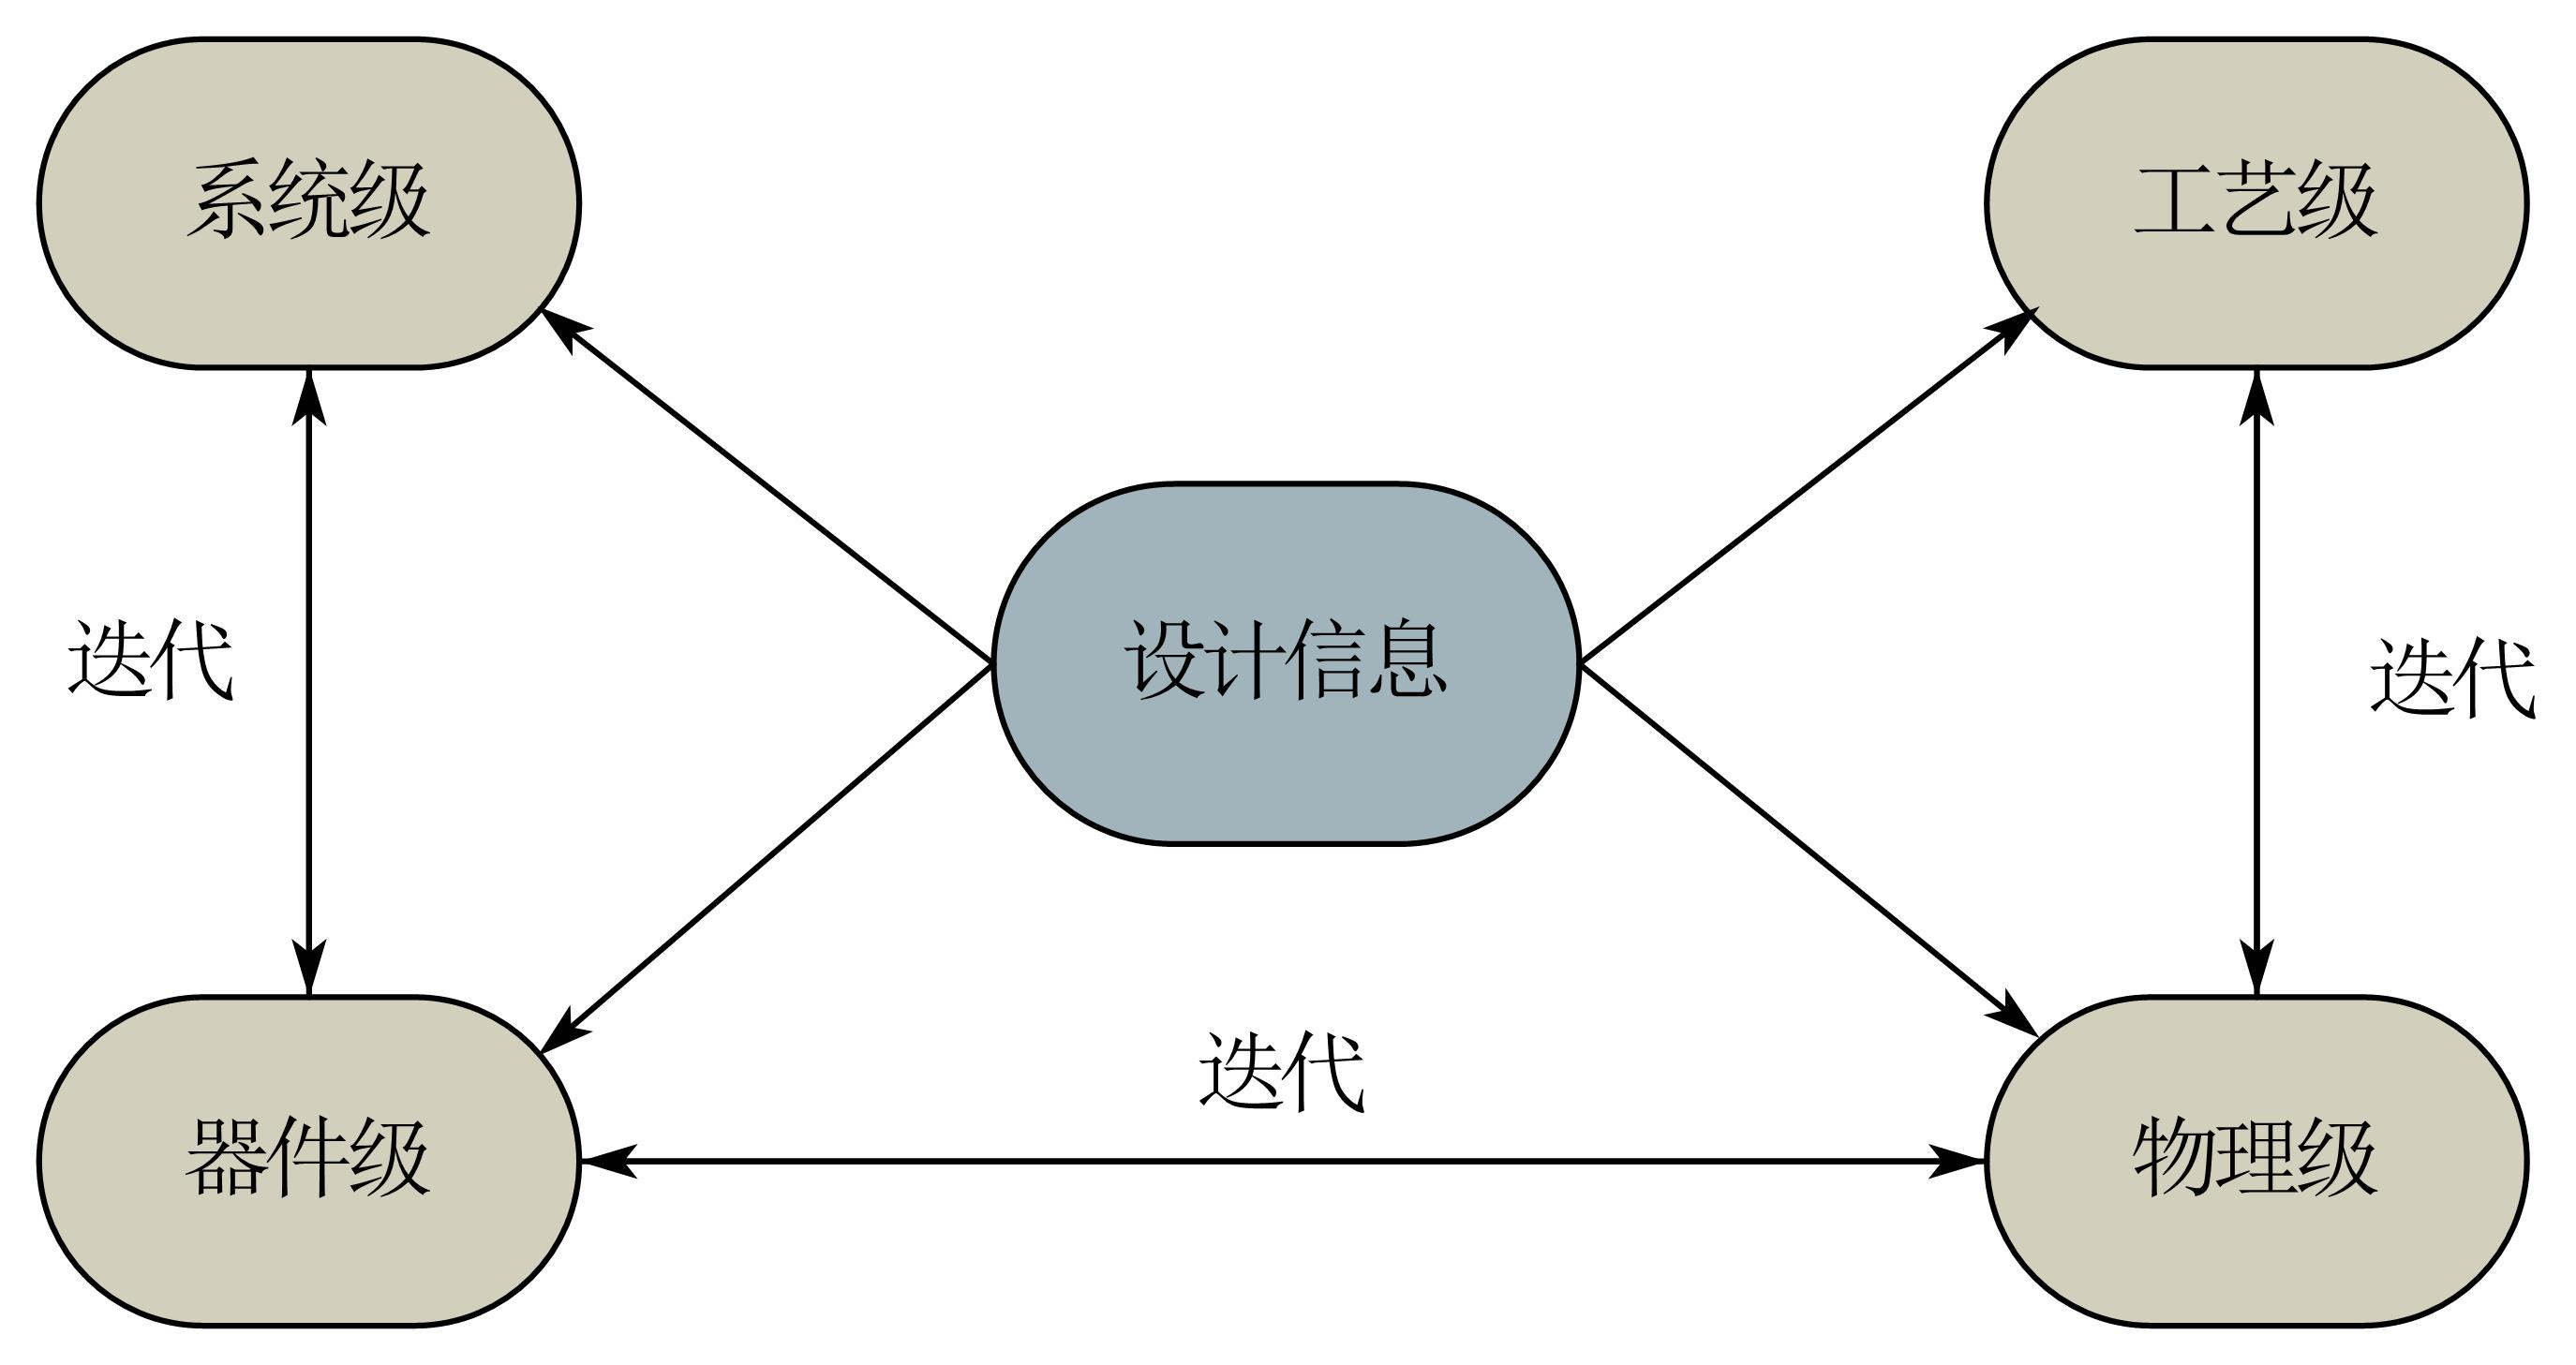
\includegraphics[width=0.7\textwidth]{fig1}
	\caption{MEMS分阶层描述}
     \label{fig1}
\end{figure}

工艺级设计关注的焦点是MEMS的几何形状的可加工制造性;与工艺级所关注的焦点不同,物理级、器件级和系统级这三个设计阶层是从不同的角度或不同的抽象阶层来研究MEMS的行为特性。物理级是从物理场的角度研究分析器件内的能量与信息转换机理;相对于物理级,器件级是从更高阶层的角度研究MEMS器件内的能量与信息的转换,在该阶层只关注MEMS器件主要的行为特性,即关注主要矛盾,忽略次要因素,以便对器件行为进行快速的设计、评估;而在系统级设计中研究分析由更多微器件(如微传感器、微致动器、接口电路等)构成微系统的整体性能,以寻求相对合理的系统整体设计方案。

分阶层的结构化设计方法是目前国际上 MEMS 设计的主流方法,因此适用于 MEMS 各阶层的建模与仿真方法是 MEMS 器件或系统设计方法和 MEMS CAD 领域的研究热点。


\subsection{工艺级}

工艺级由几何仿真和物理仿真组成。几何仿真主要从几何的角度研究版图与加工工艺所能确定 的MEMS结构是否满足设计的要求,这也是早期MEMS的bottom-up设计方法的主要内容。物理仿真 是对MEMS加工过程的物理化学变化进行仿真分析,如材料的刻蚀得到的几何形状与腐蚀时间和腐蚀液之间的关系等,可用的软件有ACES\cite{bibc24}, DROPIE等。

\subsection{物理级}

物理级主要是采用有限元分析 (Finite Element Analysis, FEA) 和边界元分析(Boundary Element Analysis, BEA) 方法以及这两种方法的结合,对微结构和静电场以及静电-结构耦合场等的行为特性进行数值仿真分析。可用于MEMS物理级设计的商品化FEA/BEA仿真器有:Intellisense\cite{bibc25}, CAEMEMS\cite{bibc26}, CFDRC\cite{bibc27}, ANSYS\cite{bibc28},  ABAQUS\cite{bibc29}, MAXWELL\cite{bibc30}, CoventorWare\cite{bibc31}, SESES\cite{bibc32}, SOLIDIS\cite{bibc33}, IntelliCAD\cite{bibc34}等。这些方法首先对机械结构或静电场进行网格划分形成描述器件行为的系统矩阵,然后结合边界条件求解系统矩阵描述的方程来实现器件行为的仿真分析。

采用FEA/BEA方法时,如果网格划分的足够精细,可以得到非常精确的仿真结果。此外,网格划分可以有多种类型,如三角形和四面体网格,可以实现对任意形状的结构进行网格化建模,因此FEA/BEA方法的适用范围较广。为了实现机械结构和静电等物理场的耦合分析,可采用松弛法\cite{bibc35}、牛顿法\cite{bibc36}、同伦法\cite{bibc37}等对器件的FEA和BEA耦合物理模型进行求解,以得到仿真结果。

FEA/BEA 方法存在以下不足:在对器件行为进行仿真分析时,如果 MEMS 器件的结构尺寸发生变化,则需要重新建模、网格划分,才能实现器件行为仿真,这延长了 MEMS 的设计迭代周期。此外,由于网格划分后形成的系统矩阵通常非常庞大,导致物理级的行为仿真需要非常长的计算时间。

\subsection{器件级}
为了避免常规 FEA/BEA 方法的不足,可对由 FEA/BEA 方法网格划分后形成的系统矩阵进行降阶,以减少系统自由度的个数,达到器件行为的快速仿真目的。通常把对系统模型进行降阶的过程称为宏建模\cite{bibc38} (macromodeling),得到的模型称为宏模型 (macromodel),也称为降阶模型 (Reduced-order model)。宏模型可插入电路仿真器,如 SPICE,SABER 等实现由微机械结构、接口电路等形成的 MEMS 系统级整体行为的仿真分析。

宏模型的获取主要有两种方法\cite{bibc39}:基于FEA/BEA方法和解析法。基于解析法的宏模型获取依靠建模人员手工推导,因此适用于结构简单的MEMS器件,而FEA/BEA可以对任何形状的微结构进行仿真分析,所以基于FEA/BEA的宏模型获取方法适用范围较广。基于FEA/BEA分析的宏模型获取方法主要有基于静态分析法\cite{bibc40}、基于模态分析法\cite{bibc41}以及这两种方法的结合,还有直接降阶法\cite{bibc42}。

\begin{enumerate}[fullwidth, label=(\arabic*), itemindent=2em]
\item  基于静态分析法:在一篇文献\cite{bibc43}中,在对微机械结构进行一系列静态仿真的基础上,对仿真结果进行多项式曲线拟合,从而得到机械结构的刚度宏模型。类似地,也可得到机械结构的集总质量宏模型和集总阻尼宏模型,这种模型也称为集总元素模型。对于机电能量转换器的集总元素模型,可在对微结构进行一系列基于边界元静电场分析的基础上通过曲线拟合定义电容与位移之间的关系,然后通过这些关系式获取由微结构间静电场所产生的静电力。最后把这些集总元素按照二阶振动系统的公式联系起来就是整个器件的宏模型。李伟剑在其博士论文\cite{bibc44}中采用这种方法对微陀螺进行了宏模型提取,从而进一步实现了微陀螺的耦合场分析。由于这些集总元素模型是系统矩阵的低阶等效,通过这种方法,可把采用FEA/BEA分析器件行为时器件的自由度由成千上万个减低到少数几个。集总元素宏模型构成的器件的宏模型可以以“黑箱”的形式插入系统级仿真器中实现MEMS系统级行为的仿真分析。

\item 基于模态分析法:模态分析法也是获取微结构的宏模型的有效方法。如在文献\cite{bibc45}中,器件的有效质量通过模态分析的特征值获取,然后进一步形成了器件的宏模型。

\item 静态和模态分析结合法:宏模型也可在FEA/BEA的静态分析和模态分析的基础上获取。该方法可克服获取系统集总元素宏模型所需要进行大量FEA/BEA仿真的不足。

\hspace{2em} 图(\ref{fig2})为一微镜的宏模型获取示例\cite{bibc46}。首先,通过有限元分析进行网格划分,然后采用“试载荷”作用在微器件的工作方向上进行模态分析以得到模态形状。根据微结构的变形计算各模态形状在变形中的贡献系数。依照其贡献系数大小对模态形状进行排序,以得到主导该结构变形的主要模态 (primary modal)。以这些主要模态的贡献系数为广义坐标,模态形状作为系统矩阵来建立器件的宏模型,最后,把每一个能量域的宏模型集合形成的模型作为整体器件的宏模型。

\begin{figure}[!htbp]
	\centering
	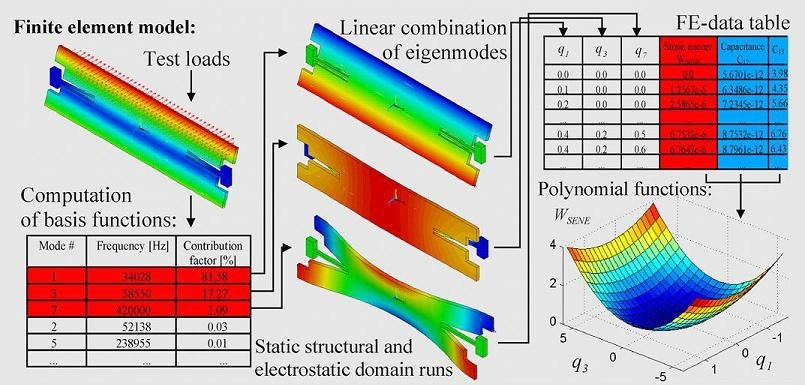
\includegraphics[width=0.95\textwidth]{fig2}
	\caption{微镜的宏模型获取}
     \label{fig2}
\end{figure}

\item 直接降阶法。如图(\ref{fig3})所示,该方法是在器件网格化后得到主导器件行为的常微分方程组基础上,直接采用数值降阶方法对该常微分方程组进行降阶,从而获取器件的降阶宏模型。降阶策略是实现该方法的关键,目前已出现的降阶策略有Arnoldi算法\cite{bibc47} 、正交分解法\cite{bibc48}(proper orthogonal decomposition, POD)、加权残值法 (Method of Weighted Residuals, MWR)\cite{bibc49}等。
\end{enumerate}

\begin{figure}[!htbp]
	\centering
	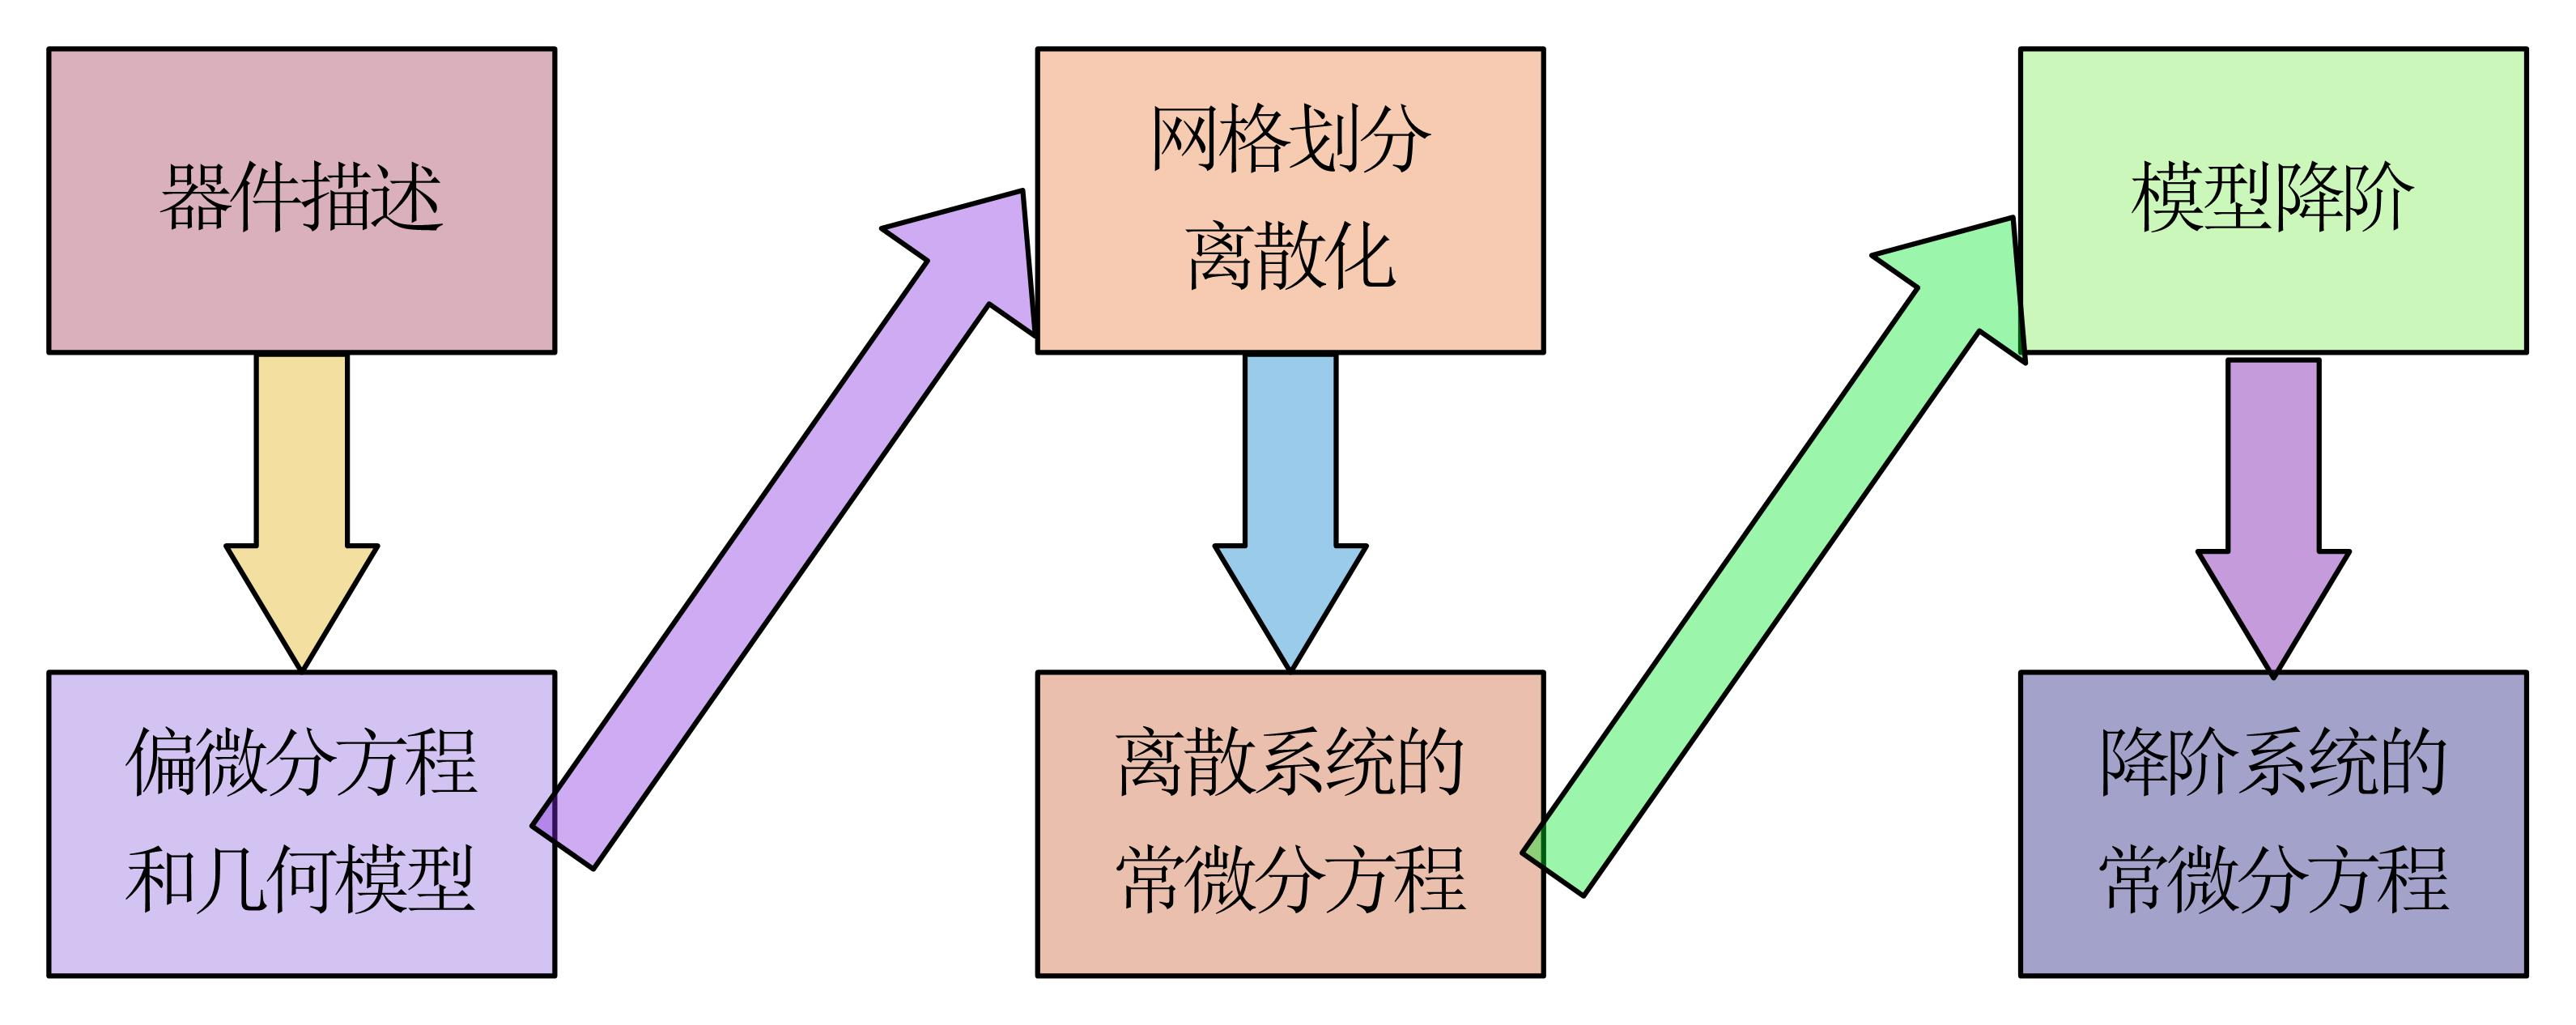
\includegraphics[width=0.8\textwidth]{fig3}
	\caption{宏模型的直接降阶获取法}
     \label{fig3}
\end{figure}

这种宏建模方法是对器件网格划分后得到的主导常微分方程组直接降阶,而器件的主导行为方程来自于有限元方法和边界元方法的网格划分结果,因此该方法不需要对器件进行FEA/BEA仿真,是目前宏模型自动获取方法的研究方向。

综上所述,基于 FEA/BEA 的宏建模方法虽然具有很高的精度,但随着器件几何拓扑和结构尺寸参数的变化,需要重新建立器件的有限元/边界元模型,然后才能获取器件的宏模型,这增加了 MEMS 的设计迭代周期。此外,采用这种方法提取宏模型首先需要建立器件的有限元/边界元模型,故该方法适合于对已有的 MEMS 器件进行宏模型提取。

\subsection{系统级}
MEMS 作为一个系统,其包含微机械、微电子、微光学、微流体等能量场以及它们的多域耦合能量场。一般来说,要实现对MEMS整体(系统级)行为的建模与仿真,理论上有两种途径:一种是通过不同物理场或不同抽象阶层的专用仿真器(如模拟、数字信号仿真器及有限元分析软件等)的耦合实现对复杂MEMS系统的仿真\cite{bibc50}。这种方法偏向于多能量域耦合的物理场分析,仿真精度高,但由于模 型的抽象层次低、模型的类型不一致,致使仿真计算代价高、收敛性差,在仿真速度上不能满足MEMS 系统级快速设计的需要;另一种是采用一种通用系统建模方法对系统中的所有子系统(或功能结构部件)进行统一建模,用一个仿真器实现对整个系统的仿真,基于这种途径的系统级设计目前有大量的应用。基于统一建模思想的MEMS建模方法有黑箱法、等效电路法、基于可重用芯核 (intellectual property, IP) 法。

①黑箱法:把前面基于 FEA/BEA 得到的宏模型以“黑箱”的形式插入电路仿真器中,实现系统整体行为的仿真分析\cite{bibc51}。在这种方法中,由于所采用的宏模型针对具有固定几何拓扑形状和尺寸参数的微器件,故适用于对已有系统行为的验证,而不便于设计迭代、优化。

②等效电路法:研究人员借助于宏观机电能量转换中的集总参数法、利用机电类似性,提出了采用电模拟的等效电路法\cite{bibc52}实现MEMS的系统级建模与仿真,到目前为止这种方法还在国内外广泛使用。简单的来说,等效电路法把机械系统位移、力、质量、弹性系数等效为电路中的电荷、电压、电感、电容,又采用变压器和回转器作为机电之间的能量转换装置。对于非线性系统建模,引入附加能量源模拟系统的非线性行为\cite{bibc53}。类似地,这种方法可向其他能量域(流体、热学等)扩展,即 采用电模拟的方法对其它能量域进行仿真与分析。这种方法虽然广泛使用,但具有以下局限性:一般难以找到与系统相适应的等效电路;受到SPICE电路仿真器基本单元类型的限制;在等效非线性系统时,需要引入附加的能量源,而这个能量源在真实系统中并不存在,故使所建模型不易理解。

为了克服上述建模与仿真方法的不足,基于可重用 IP 的设计方法为 MEMS 系统级建模与仿真提供了新思路,以期实现以下目标:高的仿真精度和建模与仿真速度;能够处理 MEMS 多能量域耦合的固有特性; 便于设计迭代和优化。

近几年来,世界各国研究机构基于可重用IP设计思想提出了不同的MEMS建模与仿真的解决方案。如国外Coventor公司的ARCHITECT\cite{bibc54}、加州大学Berkeley分校的SUGAR\cite{bibc55}、Carnegie Mellon大学的NODAS\cite{bibc56},国内西北工业大学提出的基于多端口组件网络 (Multi-Port-Element Network, MuPEN) 的 MEMS建模方法\cite{bibc57}。

这些方法的基本思想为把MEMS分解为多个功能结构部件,把这些功能结构部件建立为参数化的组件模型,组件模型按照器件的拓扑结构相互联接形成的网络表征整个MEMS。如在西北工业大学的MuPEN方法中\cite{bibc58},微加速度计可分解为接口电路和微机械器件,这些器件可进一步分解为一些基本的功能单元,见图(\ref{fig4}),把这些功能单元建立为参数化多端口组件模型,联接这些组件模型形成的网络作为整个微加速度计的系统级模型,见图(\ref{fig5})。基于该系统级模型,可以在频域和时域内仿真分析系统的整体行为特性。

\begin{figure}[!htbp]
	\centering
	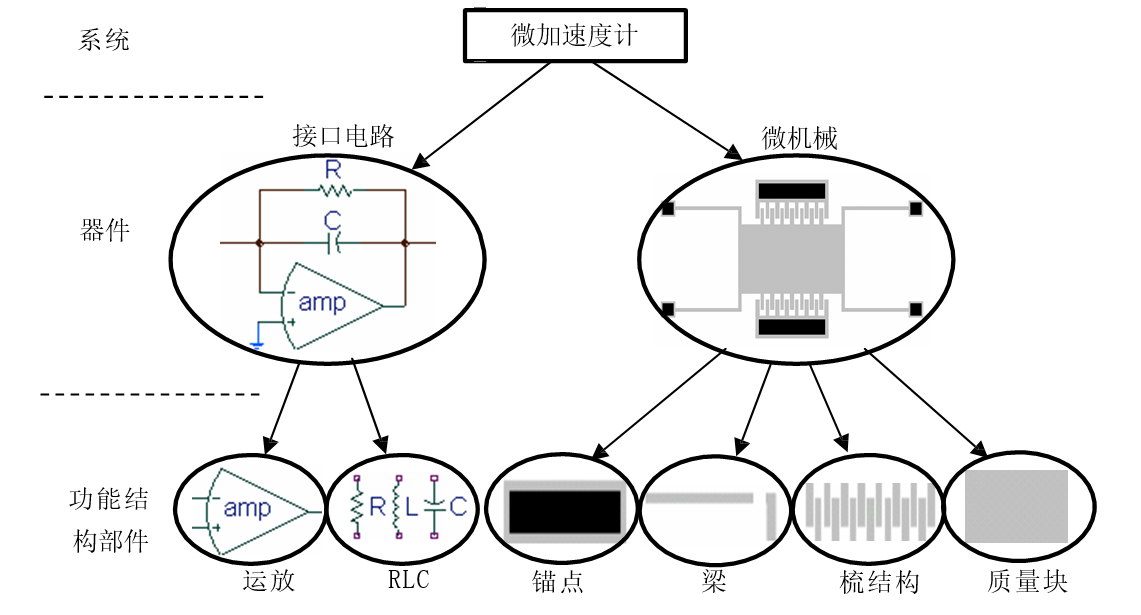
\includegraphics[width=0.95\textwidth]{fig4}
	\caption{微加速度计的分解}
     \label{fig4}
\end{figure}

\begin{figure}[!htbp]
	\centering
	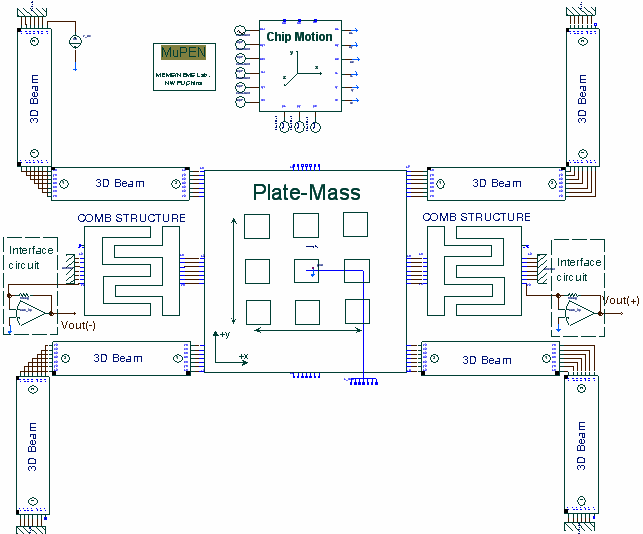
\includegraphics[width=0.9\textwidth]{fig5}
	\caption{微加速度计的多端口组件网络模型}
     \label{fig5}
\end{figure}

上述这些基于可重用 IP 设计思想的建模方法其主要区别在于模型编码语言、模型的适用范围和使用方法有所不同。SUGAR 在 MATLAB平台上建立了基于网表(Netlist) 的 MEMS 建模与仿真体系;NODAS 采用 MAST 语言在 SABER 平台上针对作平面运动的 MEMS 器件建立了基于示意图 (schematics) 形式的 NODAS 组件库,目前采用 Verilog-A 语言在 Cadence Spectre 仿真器把局限于作平面运动的组件库扩展到三维空间;ARCHITECT 也采用 MAST 语言在 SABER 平台实现了基于示意图的建模与仿真体系;而西北工业大学的 MuPEN 方法考虑到 SABER 仿真器在国内比较广泛适用,采用硬件描述语言 MAST 在 SABER 仿真平台建立了基于 schematics 形式的 MEMS 建模与仿真体系。此外,由于选择的软件平台不同,在进行模型仿真时具有的仿真分析功能不同,组件模型的差异也使得同一系统的网络模型有所不同、仿真精确度也有所不同。

\newpage
\section{关键科学技术问题}

支持微机电系统的 CAD 系统是计算机辅助设计技术与微型机电系统技术紧密结合的产物。MEMS 中的 CAD 系统跨越了机械、微电子、光学等多个领域,除了具有传统的 CAD 系统所共有的特性外,还具有自身新的特点,其中关键的科学与技术问题主要有 \cite{bibc59}:在设计时需要考虑微小尺度下的力的作用,加工方法改变对设计产生影响,材料性质的变化,加工精度及检测,与微电子系统紧密耦合,涉及多学科的设计知识。

\subsection{设计中需要考虑在微小尺度下力的作用}

一些在常规机械中很少考虑的力,例如静电力、表面张力等的作用明显增强。微型机械中起主导作用的力是表面力。在 MEMS 的设计中,动力的产生经常采用静电或压电方式。即使在采用电磁方式的情况下,由于尺度的微小,所考虑的重点也明显不同于常规尺度下的机械设计。

\subsection{加工方法改变对设计产生影响}

MEMS 器件的加工方法不同于一般的传统机械,而是大量使用光刻腐蚀、离子加工、离子注入等微电子加工技术,此外,也会采用电解、激光加工等技术。在尺寸相对较大的 MEMS部件中,也可能使用精密机械加工方法。微系统技术是在微电子技术的基础上发展起来的,使得在 MEMS 中的 CAD 系统中需要使用很多类似于微电子技术里的 CAD 系统所使用的技术。因此,在结构和工艺设计方面,MEMS 的 CAD 系统比较接近于微电子 CAD 系统。但是,在另一方面,在 MEMS 的设计中,比较偏重的是设计和制造对象的机械特性和功能。这就又使得 MEMS 中的 CAD 与常规的微电子 CAD 系统有较大的不同。微电子 CAD 系统基本注重二 维几何形状的设计和加工,对被加工材料的操作基本上只涉及表面以下很浅的范围。而在 MEMS 中所要设计和加工的对象是尺寸微小的三维机械部件。

\subsection{材料性质的变化}

尺度的减小,导致材料的晶体缺陷减小,材料强度增加,并且表现出一些在常规尺度下不显著的性质和特征。这些材料性质的变化,也会对 MEMS 的设计产生一定的影响。

\subsection{加工精度及检测}

在微系统器件的加工技术中,可达到的绝对精度提高,相对精度降低。这些特点需要在设计 CAD 系统加以考虑。同时,由于检测手段较少,对模拟和仿真的要求增强。

\subsection{与微电子系统耦合紧密}

MEMS 的研究工作一直把机电一体化集成作为一个重要的发展方向。在单个衬底或者多个衬底上集成上各类传感器、动作器、机械结构以及相应的信号处理和控制电路,对于提高 MEMS 的集成度和可靠性,增加功能,降低成本来说是非常重要的。因此,在 MEMS 中电子线路与机械部分的耦合是很紧密的。这也必然要求其 CAD 系统提供相应的支持。这样,MEMS 中的 CAD 系统既不是常规的机械 CAD 系统,也不是常规的微电子 CAD 系统。同时,它也不是两者之间的简单的相加,而是两者之间有机的结合和扩展。

\subsection{涉及多学科的设计知识}

微系统器件不仅仅是微尺度范围的三维复杂机械结构,而且涉及到光学、电子、机械、流体等多个学科领域,在设计时,每个领域内的参数都需要进行计算,才能设计出合理可靠的微系统器件,才能正确的模拟所设计的微系统器件的性能。因此,MEMS 的 CAD 系统一般有统一的算法库和数据库,用来存放各个有关学科领域的设计方法和数据。

\newpage
\section{存在的问题与发展趋势}

\subsection{高度集成化}

在过去的近 40 年中,集成电路的发展遵循摩尔定律,即按每 3 年特征尺寸减小0.7倍,集成度每 3 年翻一番规律发展\cite{bibc60}。据分析, IC 特征尺寸的指数减小规律还将继续10~20年。目前,IC 工艺已进入纳米阶段,最小已经可以达到7nm,台积电5纳米工艺正在开发中\cite{bibc61}。未来将研制生产巨大规模集成电路和单片系统集成 (System on a chip , 即 SOAC)。IC 的发展为研制生产 MEMS 提供了坚实的技术基础。
集成化智能微机电系统的发展,对CAD的集成化提出了更高的要求,未来的MEMS CAD系统将向着更高的集成度发展。

\subsection{跨平台能力}

很多MEMS CAD软件的跨平台应用能力不足, MEMS CAD系统应该向着全平台化发展,尽可能具有在几乎所有的主流操作系统上运行的能力,包括 UNIX、Mac OS、Windows 、Linux 等。

\subsection{高质量和高性能}

MEMS CAD系统需要在 CAD、CAM、三维动画和可视化仿真等领域具有高质量和高效率的图形生成能力。

\subsection{出色的编程特性}

MEMS CAD需要有严格的规范控制、良好的稳定性、良好的前瞻性、伸缩性和易使用性,以利于研发人员使用MEMS CAD系统进行编程。

\subsection{工艺设计能力}

在工艺模拟功能方面,虽然一些商业软件如MEMS Pro/CAM、Coventor、Intellisuite都支持三维工艺模拟\cite{bibc62},但是工艺的模拟和实现都是比较简单和理想化的,而且都基本没有考虑到工艺设计的内容,实质上没有工艺设计能力。而在实际的MEMS研究中,由于加工条件、设备以及工艺水平的限制,工艺设计是所有设计内容中最关键、最困难的一步!

MEMS CAD系统应以工艺为主线贯穿整个设计过程,能够实现 MEMS工艺设计的在线模拟和其他器件的性能分析与版图设计。

\newpage
% 参考文献
% 宽度9
\begin{thebibliography}{9}
\addcontentsline{toc}{section}{参考文献}

% 每条参考文献均需用<\bibitem{}>引出,
% 花括号里的内容为此条参考文献的标签,
% 可用<\cite{}>引用。
% 若参考文献条数超过99,
% 请联系作者修改.cls类文件,
% 否则空格略有不完美。
\bibitem{bibc1}  Gabriel, Kaigham; Jarvis, John; Trimmer, William (1988). Small Machines, Large Opportunities: A Report on the Emerging Field of Microdynamics : Report of the Workshop on Microelectromechanical Systems Research ; Sponsored by the National Science Foundation. AT\&T Bell Laboratories.
\bibitem{bibc2}  Waldner, Jean-Baptiste (2008). Nanocomputers and Swarm Intelligence. London: ISTE John Wiley \& Sons. p. 205. ISBN 978-1-84821-009-7.
\bibitem{bibc3}  James B. Angell; Stephen C. Terry; Phillip W. Barth (April 1983). "Silicon Micromechanical Devices". Scientific American. 248 (4): 44–55. doi:10.1038/scientificamerican0483-44
\bibitem{bibc4}  Electromechanical monolithic resonator, U.S. patent 3614677, Filed April 29, 1966; Issued October 1971
\bibitem{bibc5}  Wilfinger, R.J.; Bardell, P.H.; Chhabra, D.S. (1968). "The Resonistor: A Frequency Selective Device Utilizing the Mechanical Resonance of a Silicon Substrate". IBM J. 12: 113–8. doi:10.1147/rd.121.0113
\bibitem{bibc6}  Nathanson, H. C.; Wickstrom, R. A. (15 August 1965). "A Resonant-Gate Silicon Surface Transistor with High-Q Band-Pass Properties". Applied Physics Letters. 7 (4): 84–86. doi:10.1063/1.1754323
\bibitem{bibc7}  R. Ghodssi; P. Lin (2011). MEMS Materials and Processes Handbook. Berlin: Springer. ISBN 978-0-387-47316-1.
\bibitem{bibc8}  T. Polster; M. Hoffmann (2009). "Aluminium nitride based 3D, piezoelectric, tactile sensors". Proc. Chem. 1: 144–7. doi:10.1016/j.proche.2009.07.036
\bibitem{bibc9}  M. Birkholz; K.-E. Ehwald; P. Kulse; J. Drews; M. Fröhlich; U. Haak; M. Kaynak; E. Matthus; K. Schulz; D. Wolansky (2011). "Ultrathin TiN membranes as a technology platform for CMOS-integrated MEMS and BioMEMS devices". Adv. Func. Mat. 21 (9): 1652–1654. doi:10.1002/adfm.201002062
\bibitem{bibc10}  McCord, M. A.; M. J. Rooks (2000). "2". SPIE Handbook of Microlithography, Micromachining and Microfabrication.
\bibitem{bibc11}  Marc J. Madou, Fundamentals of Microfabrication and Nanotechnology, Volume III: From MEMS to Bio-MEMS and Bio-NEMS: Manufacturing Techniques and Applications, p. 252, CRC Press, 2011 ISBN 1439895244.
\bibitem{bibc12}  Williams, K.R.; Muller, R.S. (1996). "Etch rates for micromachining processing" (PDF). Journal of Microelectromechanical Systems. 5 (4): 256. CiteSeerX 10.1.1.120.3130. doi:10.1109/84.546406
\bibitem{bibc13}  Kovacs, G.T.A.; Maluf, N.I.; Petersen, K.E. (1998). "Bulk micromachining of silicon" (PDF). Proceedings of the IEEE. 86 (8): 1536. doi:10.1109/5.704259
\bibitem{bibc14}  Chang, Floy I-Jung (1995). Xenon difluoride etching of silicon for MEMS (M.S.). Los Angeles: University of California.
\bibitem{bibc15}  S.D. Senturia, R.M. Harris, et al. A Computer-Aided Design System for Microelectromechanical Systems. Journal of Microelectromechanical Systems. 1992, 1(1): 3-13.
\bibitem{bibc16}  F. Maseeh. IntelliCAD: the CAD for MEMS. WESCON/95 Conference Record, New York, NY, USA, 1995,pp. 320-324.
\bibitem{bibc17}  黄庆安,秦明,李伟华, 等.MEMS CAD进展[C].第六届全国敏感元件与传感器学术会议论文集.北京:东南大学,1999:13~16.
\bibitem{bibc18}  http://www.coventor.com/coventorware/
\bibitem{bibc19}  http://www.memscap.com/products-cad.html
\bibitem{bibc20}  常洪龙, 苑伟政, 马炳和. MEMS 的集成设计平台的关键技术研究.中国机械工程.2004,15(10): 916-920.
\bibitem{bibc21}  张海霞, 郭辉. MEMS CAD 系统 IMEE 的研究和开发. 微纳电子技术.2003. 40(7/8): 92-95.
\bibitem{bibc22}  S.D.Senturia, CAD Challenges for Microsensor, Microactuators, and Microsystem, Pro.IEEE, 1998,86(8): 1611-1626.
\bibitem{bibc23}  S.D. Senturia. Microsystem design. Boston: Kluwer Academic Publishers.2002.
\bibitem{bibc24}  Zachary Giano,Randolph D. Hubach,Joseph M. Currin,Denna L. Wheeler. Adverse childhood experiences and MSM marijuana use[J]. Drug and Alcohol Dependence,2019,198.
\bibitem{bibc25}  Yuhuan Du,Xiaodong Zhang,Yang Wang,Tong Mu. Design on exoskeleton robot intellisense system based on multi-dimensional information fusion[P]. Mechatronics and Automation (ICMA), 2012 International Conference on,2012.
\bibitem{bibc26}  Buser, R.A., Crary, S.B., Juma, O.S.. Integration of the anisotropic-silicon-etching program ASEP within the CAEMEMS CAD/CAE framework[P]. Micro Electro Mechanical Systems, 1992, MEMS '92, Proceedings. An Investigation of Micro Structures, Sensors, Actuators, Machines and Robot. IEEE,1992.
\bibitem{bibc27}  Lobur, M., Napieralski, A., Sviridova, T.. Application of CFDRC software for modeling of chosen microstructures[P]. Modern Problems of Radio Engineering, Telecommunications and Computer Science, 2002. Proceedings of the International Conference,2002.
\bibitem{bibc28}  Iurlova,Sevodina,Oshmarin,Iurlov. Algorithm for solving problems related to the natural vibrations of electro-viscoelastic structures with shunt circuits using ANSYS data[J]. International Journal of Smart and Nano Materials,2019,10(2).
\bibitem{bibc29}  Lina Riaño,Yoann Joliff. An Abaqus ™ plug-in for the geometry generation of Representative Volume Elements with randomly distributed fibers and interphases[J]. Composite Structures,2019,209.
\bibitem{bibc30}  Naeem Sadiq,Muhammd Imran,Constantin Fetecau,Najma Ahmed. Rotational motion of fractional Maxwell fluids in a circular duct due to a time-dependent couple[J]. Boundary Value Problems,2019,2019(1).
\bibitem{bibc31} K. Neethu,K.J. Suja. Sensitivity Analysis of Rectangular Microcantilever Structure with Piezoresistive Detection Technique Using Coventorware FEA[J]. Procedia Computer Science,2016,93.
\bibitem{bibc32}  Korvink, J.G., Funk, J., Roos, M., Wachutka, G., Baltes, H.. SESES: a comprehensive MEMS modelling system[P]. Micro Electro Mechanical Systems, 1994, MEMS '94, Proceedings, IEEE Workshop on,1994.
\bibitem{bibc33}  K. -O. Groeneveld,R. Maier,H. Rothard. De spectric electroniorum secundariorum prorsus rectorum e corporibus solidis ioniis penetrantibus inductorum[J]. Il Nuovo Cimento D,1990,12(6).
\bibitem{bibc34} Maseeh, F.. IntelliCAD: the CAD for MEMS[P]. WESCON/'95. Conference record. 'Microelectronics Communications Technology Producing Quality Products Mobile and Portable Power Emerging Technologies',1995.
\bibitem{bibc35}  Suman Dabas,Poonam Joshi,Ramesh Agarwal,Raj Kumar Yadav,Garima Kachhawa. Impact of audio assisted relaxation technique on stress, anxiety and milk output among postpartum mothers of hospitalized neonates: A randomized controlled trial[J]. Journal of Neonatal Nursing,2019.
\bibitem{bibc36}  Shougui Zhang,Yueyue Yan,Ruisheng Ran. Path-following and semismooth Newton methods for the variational inequality arising from two membranes problem[J]. Journal of Inequalities and Applications,2019,2019(1).
\bibitem{bibc37}  Shehu Maitama,Weidong Zhao. Local fractional homotopy analysis method for solving non-differentiable problems on Cantor sets[J]. Advances in Difference Equations,2019,2019(1).
\bibitem{bibc38}  Shahabeddin Vamegh Estahbanati,Rached Dhaouadi,Maher Bakri-Kassem. Macromodeling of thermally driven V-shaped MEMS actuators[J]. Mechatronics,2017.
\bibitem{bibc39}  Mohammad Reza Pashaie,Majid Mohammadi. Estimating the local and global effects of infills on steel frames by an improved macro-model[J]. Engineering Structures,2019,187.
\bibitem{bibc40}  Zigang Xu,Xiuli Du,Chengshun Xu,Jiawei Jiang,Runbo Han. Simplified equivalent static methods for seismic analysis of shallow buried rectangular underground structures[J]. Soil Dynamics and Earthquake Engineering,2019,121.
\bibitem{bibc41}  Shieh‐Kung Huang,Chin‐Hsiung Loh. Combination of decentralized sliding mode control and online wavelet analysis for control of equipment with isolation system[J]. Structural Control and Health Monitoring,2019,26(5).
\bibitem{bibc42}  Xiaoyong Lu, Liqing Li, Xiaogang Zhou. Reduction Method of Order-Cycle Column Remove Based on Indiscernibility Relation[P]. INC, IMS and IDC, 2009. NCM '09. Fifth International Joint Conference on,2009.
\bibitem{bibc43}  N. R. Swart, S. F. Bart, et.al. AutoMM: Automatic Generation of Dynamic Macromodels for MEMS Devices. Proceedings of the IEEE Micro Electro Mechanical Systems. .1998: 178-183.
\bibitem{bibc44}  李伟剑. 微机电系统的多域耦合分析和多学科设计优化. [博士学位论文].西安:西北工业大学.
\bibitem{bibc45} D.F. Ostergaard, M. Gyimesi. Finite Element Based Reduced Order Modeling of MicroElectroMechanical Systems (MEMS). The 2000 International Conference on Modeling and Simulation of Microsystems (MSM2000). San Diego, CA, USA. 2000: 684-687.
\bibitem{bibc46}  L.D. Gabbay, S.D. Senturia. Automatic Generation of Dynamic Macro-Models Using Quasi-Static Simulations in Combination with Modal Analysis. Technical Digest. Solid-State Sensor and Actuator Workshop. Cleveland, OH, USA. 1998: 197-200.
\bibitem{bibc47}  Y. Chen, J. White. A Quadratic Method for Nonlinear Model Order Reduction. Proceedings of the International Conference on Modeling and Simulation of Microsystems, MSM’2000. San Diego, CA, USA. 2000: 27-29.
\bibitem{bibc48}  J. Chen, S.-M. Kang. Model-order reduction of nonlinear MEMS devices through arclength-based Karhunen-Loeve decomposition. Proceedings of IEEE International Symposium on Circuits and Systems. Sydney, NSW. 2001, 3: 457-460.
\bibitem{bibc49}  Geng Jian, Zhang Linghua. A time-difference-of-arrival location method based on residual sorting and weighted matrix amended[P]. Wireless Communications and Signal Processing (WCSP), 2011 International Conference on,2011.
\bibitem{bibc50}  Huo Pengfei, Yuan Weizheng, Li Weijian. Analytical Model of Micro-mechanical Components for MEMS System-level Simulation Using Euler Parameters Method. Asia-Pacfic Confrence of Transducers and Micro-Nano Technology2004. Sapporo, Japan. 2004. 3-2. 955-959.
\bibitem{bibc51}  Lei Tang,Fang Yang,Xianyong Feng. A novel method for distribution system feeder reconfiguration using black-box optimization[P]. ,2013.
\bibitem{bibc52}  Ze Yu,GuiZhen Lu. Equivalent circuit method for analyzing high impedance surface based microwave absorbing structure[P]. General Assembly and Scientific Symposium (URSI GASS), 2014 XXXIth URSI,2014.
\bibitem{bibc53}  T. Veijola. Nonlinear Circuit Simulation of MEMS Components: Controlled Current Source Approach. Proceedings of ECCTD'01. Espoo, Finland. 2001,3: 377-380.
\bibitem{bibc54}  G. Lorenz, A. Morris, I. Lakkis. A Top-Down Design Flow for MOEMS. DTIP 2001.
\bibitem{bibc55}  Zhou, Ningning. Simulation and synthesis of MicroElectroMechanical systems. University of California, Berkeley. PhD Thesis.2002.
\bibitem{bibc56}  Wong, G.C., Tse, G.K., Jing, Q., Tamal Mukherjee, Fedder, G.K.. Accuracy and composability in NODAS[P]. Behavioral Modeling and Simulation, 2003. BMAS 2003. Proceedings of the 2003 International Workshop on,2003.
\bibitem{bibc57}  霍鹏飞, 苑伟政, 马炳和. MEMS 惯性传感器的系统级建模技术研究.西北工业大学学报.2004,22(4): 403-407.
\bibitem{bibc58}  霍鹏飞, 马炳和, 苑伟政. 一种基于多端口组件网络的 MEMS 系统级建模方法. 机械科学与技术.2005,24(2): 192-195.
\bibitem{bibc59}  俞武嘉,李建华,傅建中,陈子辰.面向MEMS的CAD显示设计研究[J].机电工程,2001(05):78-80.
\bibitem{bibc60}  刘光辉,亢春梅.MEMS技术的现状和发展趋势[J].传感器技术,2001(01):52-56.
\bibitem{bibc61}  电子说:http://www.elecfans.com/d/874658.html,访问日期:2019年4月7日.
\bibitem{bibc62}  张海霞,郭辉,肖志勇, 等.MEMS CAD系统 IMEE的研究和开发[C].//中国微米/纳米第六届学术年会论文集.北京大学,2003:92-95.

\end{thebibliography}

\end{document} 